

% TODO aktuell das ganze db.tex war nicht dabei





% TODO ab hier 
%------------------------------------------------------------------------------


%------------------------------------------------------------------------------
\begin{frame}{Set theory for databases}
Source: Gunter Vasold, \emph{Datenbanken} class (SS 2017)\medskip 

    % ----------------------------------------------
  \begin{columns}[T,onlytextwidth]
  \metroset{block=fill}
    \column{0.52\textwidth}
    \begin{exampleblock}{Relational databases = related tables}\footnotesize
        Eine relationale Datenbanken bestehen aus Tabellen als Darstellungsform von Relationen:
\begin{enumerate}\scriptsize
    \item Jede Tabelle entspricht einem abzubildenden Entitätstyp
    \item Jede Zeile einer Tabelle entspricht einer Entität (e.g. einem bestimmten Buch)
    \item Jede Spalte einer Tabelle entspricht einem Attribut
    \item Jedes Attribut (d.h. jede Spalte) hat einen bestimmten Datentyp
\end{enumerate}
    \end{exampleblock}
    % ----------------------------------------------
    \column{0.41\textwidth}
      \metroset{block=fill}
      \begin{block}{}
      \centering 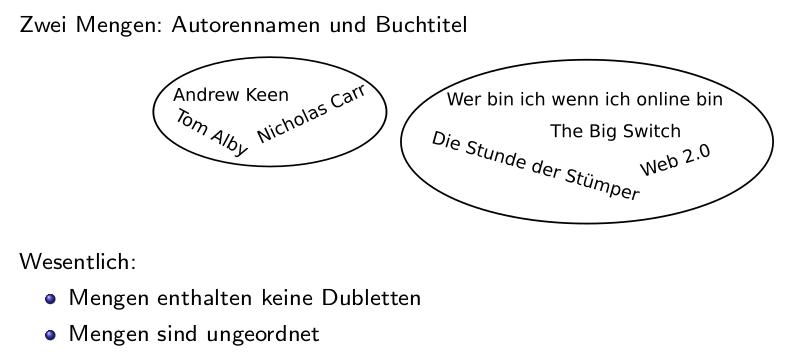
\includegraphics[width=0.9\textwidth]{img/mengen-vasold1.png}
      \end{block}

      \begin{block}{}
      \centering 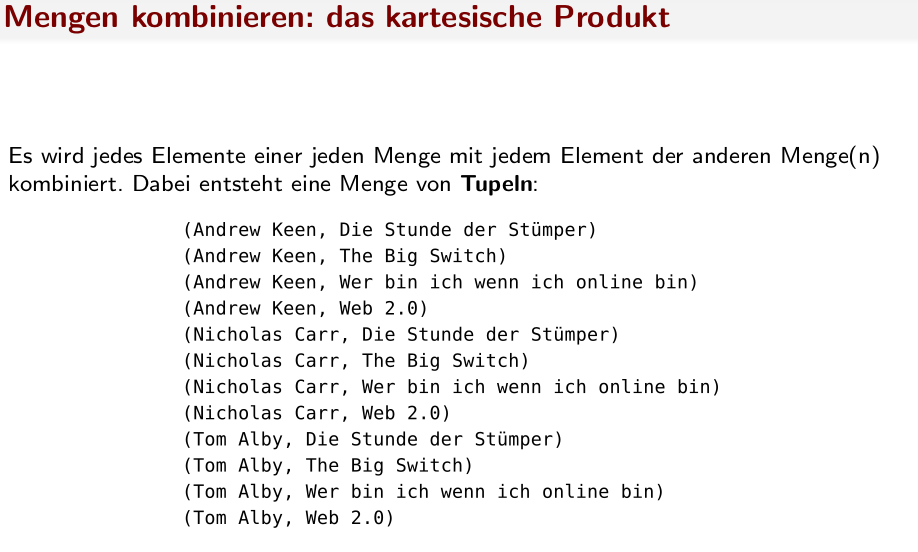
\includegraphics[width=0.9\textwidth]{img/mengen-vasold2.png}
      \end{block}
  \end{columns}
  \footnotesize
In relationalen Datenbanken werden Tabellenzeilen verschiedener Tabellen über
Primär- and Fremdschlüssel miteinander verknüpft.
Diese Beziehungen werden also nicht in der Datenbank gespeichert, sondern erst
im Zuge der Abfrage durch Wertevergleich konstruiert.
\end{frame}


%------------------------------------------------------------------------------
\begin{frame}{Mengenlehre and Relationen}
\small 
Quelle: Gunter Vasold, DB-LV 2017 
  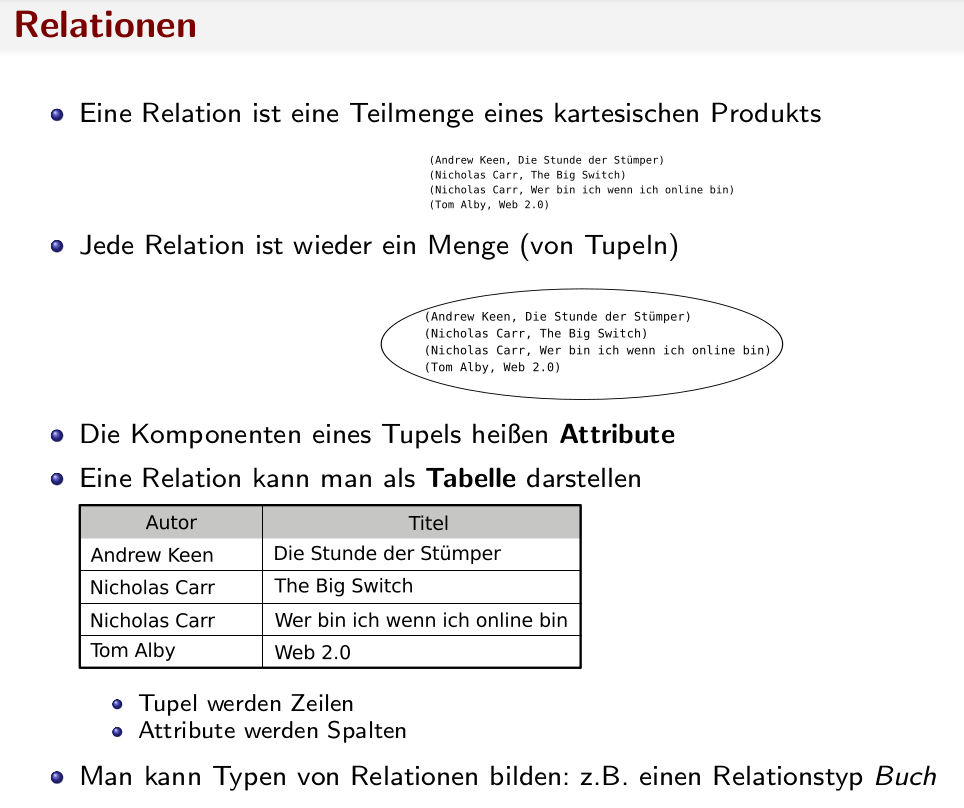
\includegraphics[width=0.8\textwidth]{img/menge-vasold3.png}
\end{frame}


